\documentclass[a4paper,12pt]{article}
\usepackage[MeX]{polski}
\usepackage[utf8]{inputenc}
\usepackage{graphicx}

%opening
\title{Todd Helton}
\hline
\author{}

\begin{document}

\maketitle
\centering
\begin{tabular}{||lr||}
\hline
Todd Helton&\\
\end{tabular}

\begin{tabular}{lr}
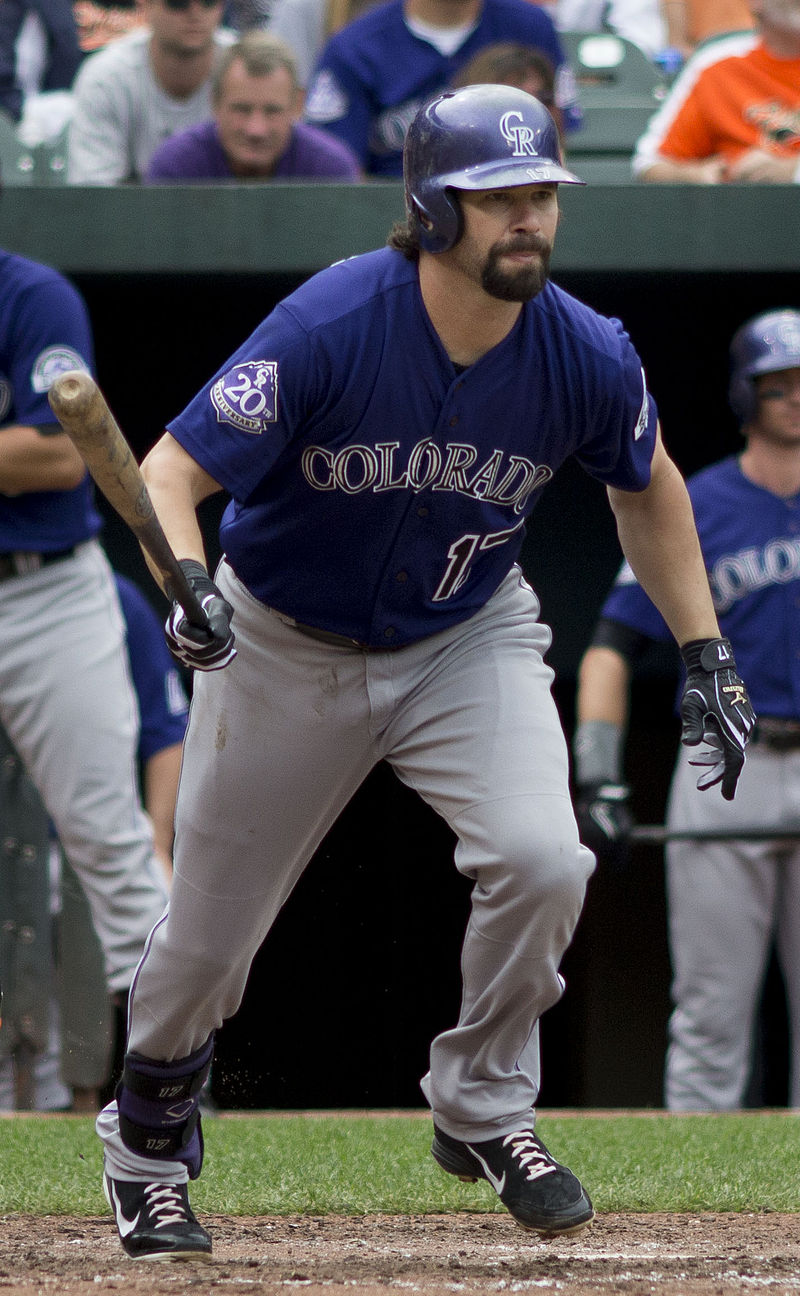
\includegraphics[scale=0.15]{ziomek.jpg}&\\
\end{tabular}
\begin{tabular}{||lr||}
\hline
 Pierwszobazowy&\\
\hline
Pełne imię i nazwisko & Todd Lynn Helton\\
\hline
 Pseudonim &  	The Toddfather\\
\hline
 Data  & 2014\\
\hline
 Miejsce urodzenia&	20 sierpnia 1973\\
\hline
 Odbijał &  	lewą\\
\hline
 Rzucał &  	lewą\\
\hline
 Debiut &  	2 sierpnia 1997\\
\hline
 Ostatni występ & 29 września 2013\\
\hline
 Statystyki&\\
\hline
 Średnia uderzeń& 0,316\\
\hline
 Home runy&  	369\\
\hline
Uderzenia&  	2519\\
\hline
RBI&  	 	1406\\
\hline
Kariera klubowa&\\
\hline
Lata&Kluby\\
\hline
1997–2013&Colorado Rockies\\
\hline
\end{tabular}



\begin{itemize}
\item
Todd Lynn Helton (ur. 20 sierpnia 1973) --- amerykański baseballista, który występował na pozycji pierwszobazowego.
\item
Helton studiował na University of Tennessee, gdzie w latach 1992–1995 grał w baseballowej i futbolowej drużynie uniwersyteckiej Tennessee Volunteers. W rozgrywkach college baseball grał na pozycjach pierwszobazowego i miotacza. W 1995 otrzymał nagrodę Dick Howser Trophy dla najlepszego baseballisty w NCAA.
\item
W czerwcu 1995 został wybrany w pierwszej rundzie draftu z numerem ósmym przez Colorado Rockies i początkowo występował w klubach farmerskich tego zespołu, między innymi w Colorado Springs Sky Sox, reprezentującym poziom Triple-A. W Major League Baseball zadebiutował 2 sierpnia 1997 w meczu przeciwko Pittsburgh Pirates, w którym zdobył home runa i zaliczył single’a. W 1998 w głosowaniu na najlepszego debiutanta zajął 2. miejsce za Kerrym Woodem z Chicago Cubs.
\item
19 czerwca 1999 w meczu z Florida Marlins zaliczył cycle jako trzeci zawodnik w historii klubu. W 2000 po raz pierwszy zagrał w Meczu Gwiazd, uzyskał najlepszą średnią w MLB (0,372), zaliczył najwięcej w MLB RBI (147), double’ów (59), najwięcej uderzeń w National League (216) i został wyróżniony spośród pierwszobazowych otrzymując po raz pierwszy w karierze nagrodę Silver Slugger Award[2]. W kolejnych czterech sezonach cztery razy był członkiem NL All-Star Team, trzy razy zdobywał Złotą Rękawicę i trzy razy Silver Slugger Award. W 2001 wyrównał klubowy rekord Larry’ego Walkera, zdobywając w sezonie zasadniczym 49 home runów.
\item
16 września 2007 w spotkaniu z Florida Marlins zdobył 300. home runa, zaś 1 września 2013 w meczu przeciwko Cincinnati Reds zaliczył 2500. uderzenie w MLB. Po raz ostatni zagrał 29 września 2013 w meczu z Los Angeles Dodgers.
\item
17 sierpnia 2014 przed rozpoczęciem meczu Colorado Rockies – Cincinnati Reds wziął udział w ceremonii zastrzeżenia numeru 17, z którym występował.
\end{itemize}

\begin{tabular}{||l||r||}
\hline
Nagroda/wyróżnienie & Lata\\
\hline
 5{x} All-Star & 2000, 2001, 2002, 2003, 2004\\
\hline
 3{x} Gold Glove Award & 2001, 2002, 2004\\
\hline
 4{x} Silver Slugger Award & 2000–2003\\
\hline
 17 zastrzeżony przez Rockies & 2014\\
\hline
\end{tabular}

\end{document}

